 % -*- encoding: UTF8 -*-
%
%%*****************************************************************************
%%				Fabrication and Assembly										                                        
%%*****************************************************************************
\chapter{Fabrication and Assembly}
\label{Ch:Fab}	



\begin{figure}[h!]\centering 
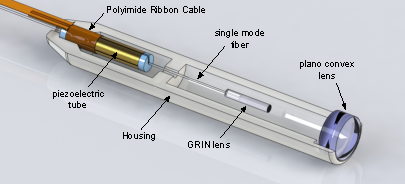
\includegraphics[width=\columnwidth]{figures/40_Fabrication/overview.pdf}
      \caption{\textbf{a)} CAD of the single modality demonstrator for testing the fiber scanner design and evaluation of the optical performance of the designed OCT beam path. }
      \label{fig:overview}
\end{figure}

The final assembly of the compact fiber scanner is shown in Figure \ref{fig:overview}. The piezoelectric actuator with four outer gold electrodes to control the lateral movement of the scanner is supplied by PI Ceramic. The addressing of the four electrodes of the piezoelectric tube is realized by a polyimide-based ribbon cable, which is wrapped around the piezoelectric tube. Conductive glue is applied through via holes in the ribbon cable to enable the connection between the platinum in the ribbon cable and the gold pads of the piezoelectric actuator. The single mode fiber is centered in the piezoelectric tube and the GRIN lens attached to it using optical adhesive. This arrangement enables a compact fiber scanner with a total length of 9mm and a resonance frequency of 750 Hz optimized for an OCT system with an A-Scan repetition rate of 100 kHz.

%\begin{figure}[h!]\centering 
%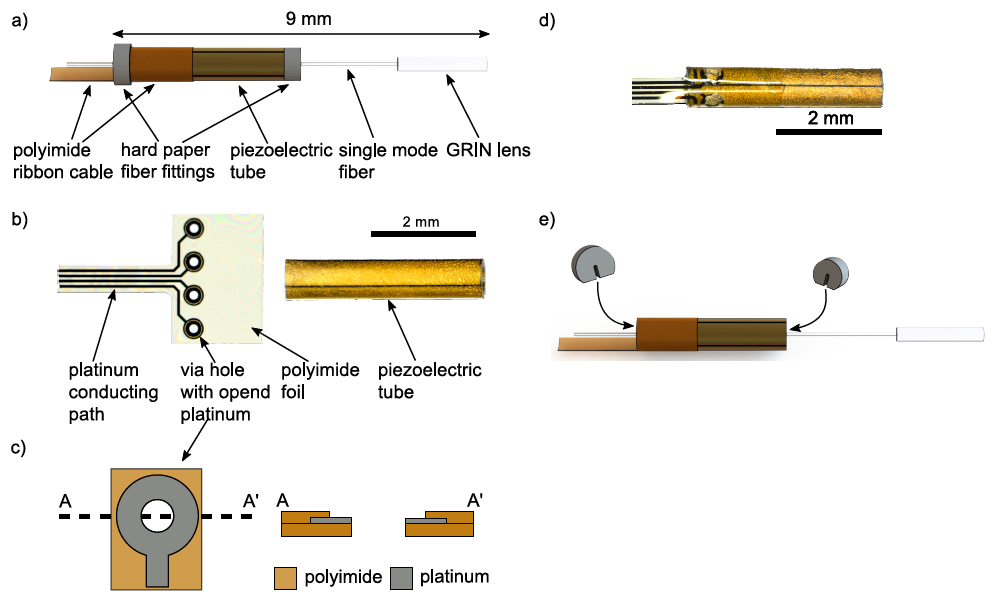
\includegraphics[width=\columnwidth]{figures/40_Fabrication/assembly.PNG}
%      \caption{\textbf{a)} True scale schematic of the designed piezoelectric fiber scanner. 
%       \textbf{b)} Photo of the polyimide ribbon cable with four vias to contact the four gold electrodes of the piezoelectric tube. The polyimide cable is manufactured in a clean room process. 
%       \textbf{c)} Schematic of one via and its cross section. The platinum around the via is partly uncovered to improve the electrical connection between the cable and the piezoelctric tube. 
%       \textbf{d)} Photo of a polyimide ribbon cable, wrapped around the piezoelectric tube that is electrical connected through the vias by conductive glue. 
%       \textbf{e)} Assembly process of the silicon fittings to center the single mode fiber inside the piezoelectric tube. The fiber is placed in the tube first. In the next step the fittings are placed in the tube and both fiber and fittings are fixed with Araldite 2020.}
%      \label{fig:assembly}
%\end{figure}


%%*****************************************************************************
\clearpage
\section{Polyimide Electrodes}
%%*****************************************************************************
Due to the small diameter of the piezoactuator, contacting its electrodes reliably is not trivial. Other piezoscanner implementations use hot welding and insulated copper wires \cite{Lee2010}, \cite{Meinert}, \cite{Huo2010}. The welding process increases significantly the diameter of the actuator, as a solder blob is needed. Furthermore, it requires welding by hand in a \SI{600}{\micro\meter} curved electrode -- not for the faint-hearted.

\begin{figure}[h!]\centering 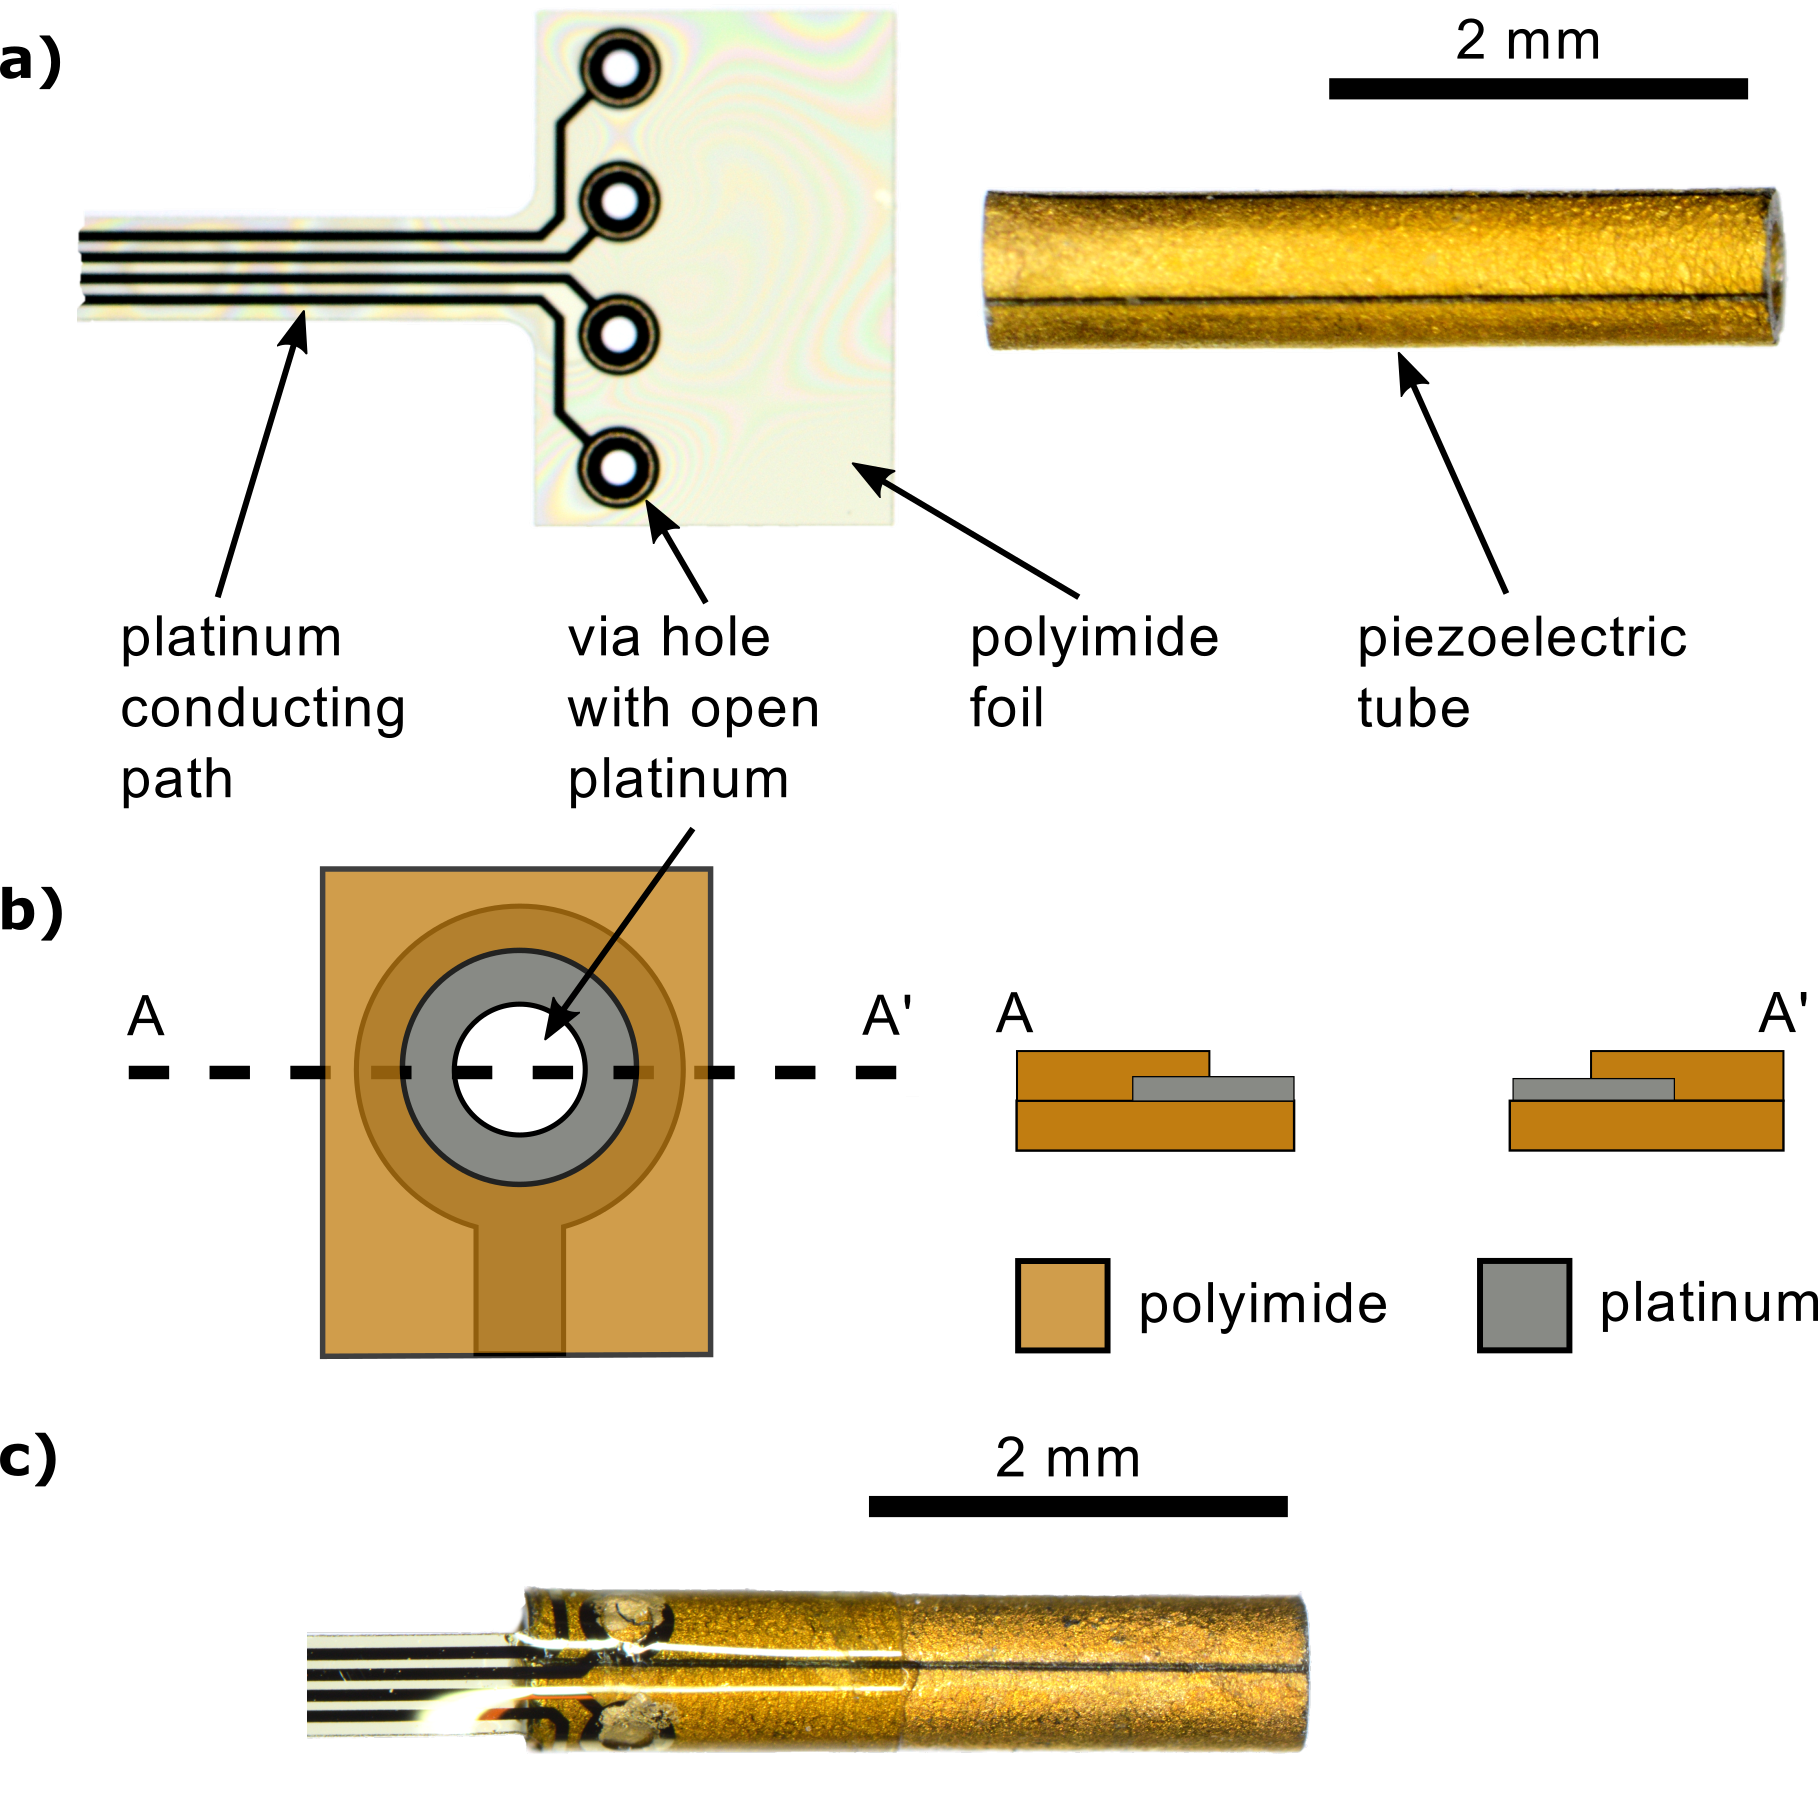
\includegraphics[width=10cm]{figures/40_Fabrication/PI/tubeFoil.pdf}
      \caption{\textbf{a)} Left: Photo of the polyimide ribbon cable with four vias to contact the four gold electrodes of the piezoelectric tube. Right: Piezotube.
      \textbf{b)} Schematic of one via and its cross section. The platinum around the via is partly uncovered to improve the electrical connection between the cable and the piezoelctric tube.
      \textbf{c)} Photo of a polyimide ribbon cable, wrapped around the piezoelectric tube that is electrical connected through the vias by conductive glue.}
      \label{fig:piRolled}
\end{figure}

Instead, we developed a polyimide ribbon cable which addresses the 4 external electrodes of the piezotube using a cleanroom process similar to the one used for cuff electrodes for nerve stimulation \cite{Rodriguez2000}. This cable consists of platinum tracks and via holes embedded in a polyimide substrate, as shown in Figure \ref{fig:piRolled}.
On one end the foil is cable is shaped to fit a zero insertion force (ZIF) connector. The other end can be rolled around the piezotube, allowing the bonding to its gold electrodes using conductive glue (Araldite 2020 with 80\% wt. silver particles).


\subsection{Cleanroom processing}
The polyimide ribbon cables are manufactured and singulated at wafer level. The process involves spincoating a \SI{5}{\micro\meter} layer of polyimide, over which \SI{100}{\nano\meter} of platinum is sputtered and then patterned by liftoff, defining the conductive traces. Finally, the vias, openings and external shape are patterned through reactive ion etching (RIE). This process is described in Figure \ref{fig:piProcess}.


\begin{figure}[h!]\centering 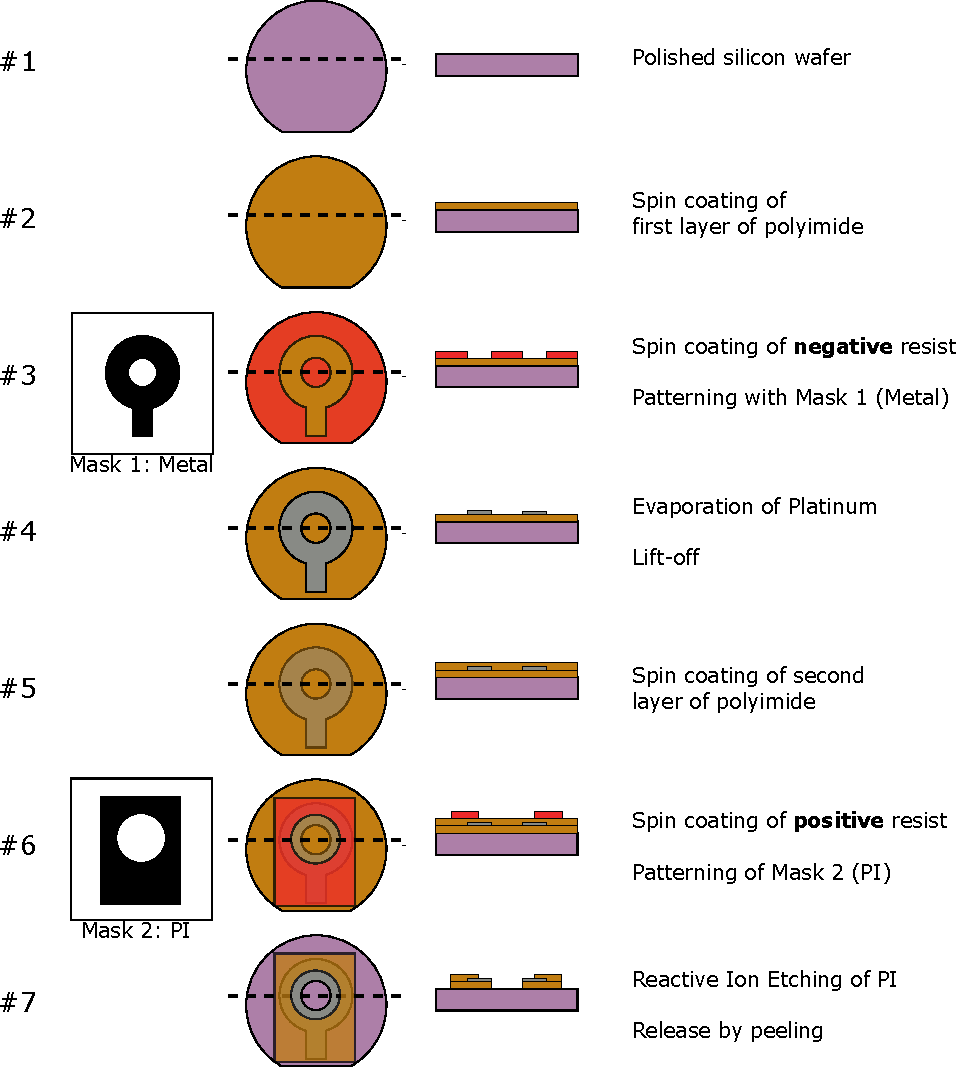
\includegraphics[width=10cm]{figures/40_Fabrication/PI/processV.pdf}
      \caption{Cleanroom fabrication process for PI electrodes.}
      \label{fig:piProcess}
\end{figure}
%
%\subsection{Bonding}
%Materials and interfaces
%\begin{figure}[h!]\centering 
\includegraphics[width=10cm,draft]{figures/foo.png}
%      \caption{Bonding cross section}
%      %\label{}
%\end{figure}

%%*****************************************************************************
\clearpage
\section{Fiber-GRIN Bonding}
%%*****************************************************************************
\begin{figure}[h!]\centering \includegraphics{figures/40_Fabrication/FiberGRIN/fiberGRINglue.pdf}
      \caption{Fiber and GRIN lens in silicon alignment tool before (a) and after (b) bonding with UV-curable adhesive.}
      \label{fig:fiberGRINglue}
\end{figure}

The GRIN lens and the end of the fiber have to be bonded together mechanically and optically for the proper functioning of the probe. This interface is critical: first, because it is subjected to very high forces due to the oscillation of the scanner, and second, because any angular or displacement error would degrade the optical quality, and third, because of the possible backreflections (See Chapter ?). 

To overcome these challenges, we align the fiber to the GRIN lens using a custom made, KOH-etched silicon alignment tool. The angled walls and high repeatibility of the KOH grooves allow the precise angle and position control of the cylindrical fiber and GRIN lens. Once in place, we apply a drop of optical UV-curable glue (NOA 76), which thanks to its wetting behavior and surface tension, creates a symmetrical wedge which provides with superb mechanical integrity.


\begin{figure}[h!]\centering 
\includegraphics[width=10cm,draft]{figures/foo.png}
      \caption{Cross section with dimensions}
      %\label{}
\end{figure}


%%*****************************************************************************
\clearpage
\section{3D Printed Housing}
%%*****************************************************************************
\begin{figure}[h!]\centering \includegraphics[width=\columnwidth]{figures/40_Fabrication/Housing/housing.pdf}
      \caption{CAD (a) and photography (b) of the single modality probe with alignment features.}
      \label{fig:housing}
\end{figure}

In order to assess the OCT imaging of the bimodal microendoscope, a single mode demonstrator was designed and built. Although the bimodal probe is designed to be assembled using the silicon bench technology, we assembled the demonstrator in a 3D printed plastic housing with no degradation to the optical quality. This is possible because the most critical alignment -- fiber to GRIN -- is performed beforehand. The rest of the components allow relatively high placement tolerances, as the beam is collimated in the region between GRIN lens and objective lens. This way, simple alignment structures which are printed with the housing allow the proper placement of all the components. 

(Material, printer, process?)

For example, in order to center the piezotube in the housing, first the fiber is retracted so that the GRIN lens seats in the GRIN alignment structure. This way the piezotube is aligned and after being glued, it is possible to push the fiber so that the GRIN is at its proper distance. 


%%*****************************************************************************
\clearpage
\section{Assembly}
%%*****************************************************************************
\begin{figure}[h!]\centering 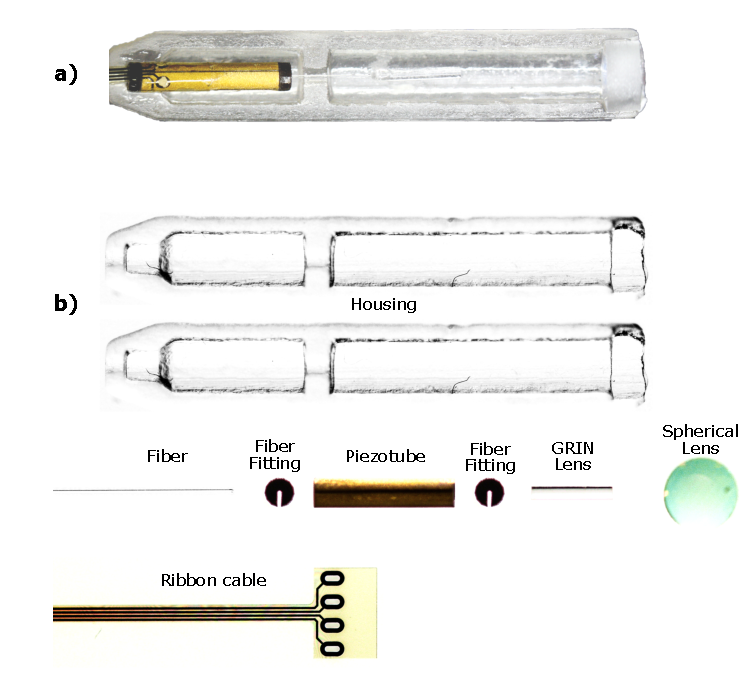
\includegraphics{figures/40_Fabrication/Assy/exploded.pdf}
      \caption{Exploded view of the components of the single modality probe.}
      \label{fig:exploded}
\end{figure}
The assembly process is summarized as follows:

\begin{enumerate}
\item The GRIN lens is bonded to the end of the fiber.
\item The GRIN lens assembly is slide through the piezotube and centered with FR-2 (synthetic resin bonded paper) fittings, which are glued to the piezotube using cyanocrilate.
\item The piezotube assembly is placed in the housing and glued in place using cyanocrilate with help of the alignment structures.
\item The planoconvex lens is placed in the bottom half of the housing and glued using UV-curable optical glue.
\item The probe is closed with the top half of the housing and sealed with UV-curable glue.
\end{enumerate}

